% Introduction

\chapter{Introduction} % Main chapter title
\label{Introduction} % For referencing the chapter elsewhere, use \ref{Chapter1} 

\hyphenation{area}
\hyphenation{areas}

\startcontents[chapters]
\Mprintcontents

%----------------------------------------------------------------------------------------

% Define some commands to keep the formatting separated from the content 

%----------------------------------------------------------------------------------------


\section{Study of forested areas}
Forests are an important component of planet's life.They are defined as large area dominated by trees. Hundreds of other definitions of forest are used throughout the world, incorporating factors such as tree density, tree height, land use, legal standing and ecological function \citep{schuck2002compilation,achard2009vital}. Forests cover about four billion hectares, or approximately 30 percent of the world's land area (see Figure~\ref{fig:forest_in_world}).

\begin{figure}[htbp]
\begin{center}
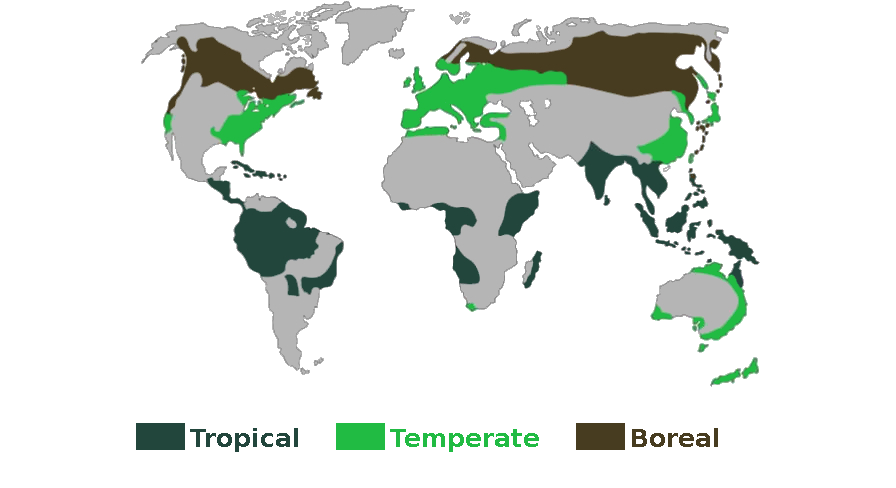
\includegraphics[width=\textwidth]{Figures/forest_in_world}
\caption{Forest repartition in the world.}
\label{fig:forest_in_world}
\end{center}
\end{figure}

Forests at different latitudes and elevations form distinctly different ecozones: boreal forests near the poles, tropical forests near the equator and temperate forests at mid-latitudes (see Figure~\ref{fig:forest_in_world}). Higher elevation areas tend to support forests similar to those at higher latitudes, and amount of precipitation also affects forest composition. Since these ecozones are very different, the study of forested areas must be restricted to a single ecozone at a time.

Forests are the dominant terrestrial ecosystem of Earth, and are distributed across the globe \citep{pan2013structure}. Forests account for 75\% of the gross primary productivity of the Earth's biosphere, and contain 80\% of the Earth's plant biomass \citep{pan2013structure}. They also hold about 90\% of terrestrial biodiversity.

Forests are also benefit for the environment; they capt and store the CO$_{2}$ \citep{fahey2010forest}. About 45\% of the total global carbon is held by forests. They also filter dust and microbial pollution of the air \citep{smith2012air}. Finally, They also play an important role in hydrological regulation and water purification \citep{lempriere2008importance} (see Figure~\ref{fig:carbon_cycle}).

\begin{figure}[htbp]
\begin{center}
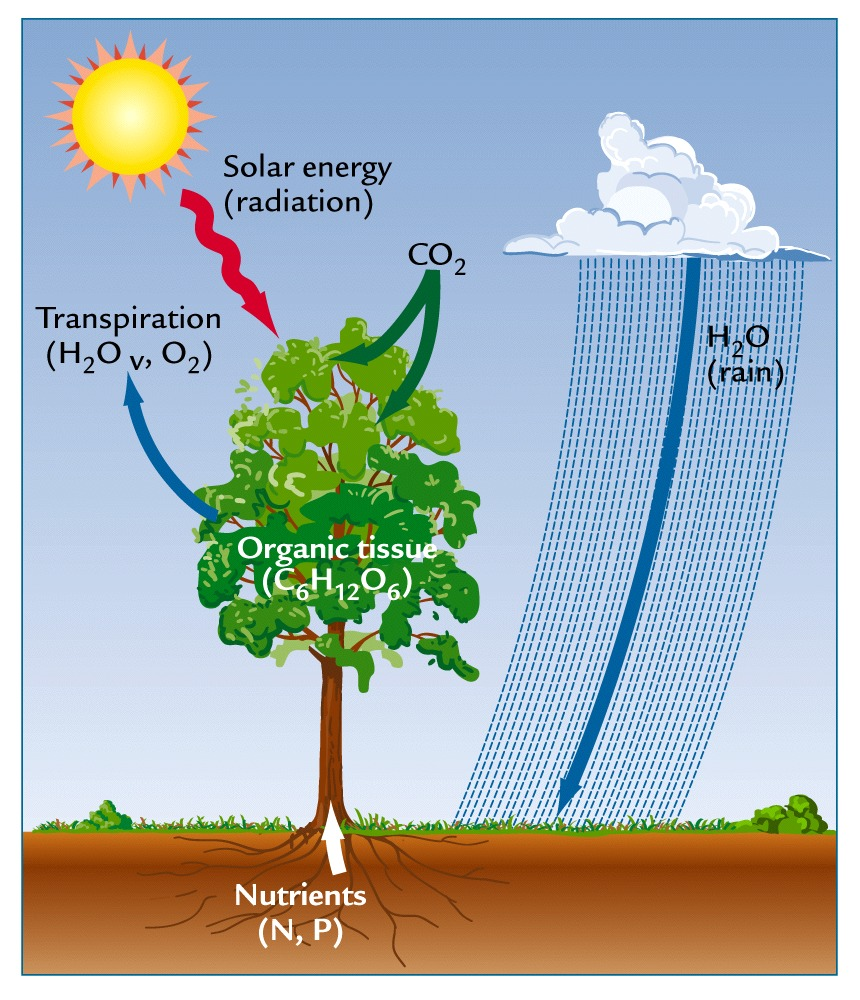
\includegraphics[width=0.5\textwidth]{Figures/carbon_cycle}
\caption{Carbon cycle: a process of CO$_{2}$ storage, water and air purification.}
\label{fig:carbon_cycle}
\end{center}
\end{figure}


Human society and forests influence each other in both positive and negative ways \citep{vogt2006global}. Forests provide ecosystem services to humans and serve as tourist attractions. Forests can also affect people's health. Human activities, including harvesting forest resources, can negatively affect forest ecosystems. Wood from forest has many uses. It has been widely used for fuel \citep{sterrett1994alternative}. In this case, hardwood is preferred over softwood because it creates less smoke and burns longer.  Wood is still an important construction material \citep{ramage2017wood}: Elm was used for the construction of wood boats. In Europe, oak is still the the wood of choice for all wood constructions, including beams, walls, doors, and floors. A wider variety of woods is also used such as poplar, small-knotted pine, and Douglas fir. Wood is also needed in the paper industry since wood fibers are an important component of most paper. Eventually, wood is also extensively used for furniture or for making tools or music instruments.

Forest are complex structures \citep{pommerening2002approaches}, for which informations are needed for management. The information can be the tree species or the tree maturity of the forest. There are two ways to extract such information from forest; field inventory or remote sensing. The field inventories are very expensive to set up and are also not adapted for a national study. A more adapted to obtain such information is remote sensing since it allows to extract them at a large scale. \\

\section{Remote sensing for forested areas}

The analysis of forested areas from a remote sensing point of view can be performed at three different levels: pixel, object (mainly trees) or stand. In statistical national forest inventory (NFI), an automated and accurate tree segmentation is needed in order to extract tree level features (basal area, dominant tree height, etc., \citep{means2000predicting,Malatamo}). However, the tree level is not the only reliable level of analysis for forest studies. When a joint mapping and statistical reasoning is required (e.g., land-cover (LC) mapping and forest inventory), forest stands remain the prevailing scale of analysis \citep{means2000predicting,White2016CJRS}. A stand can be defined in many different ways in terms of homogeneity: tree specie, age, height, maturity, and its definition varies according to the countries. \\

From a remote sensing point of view, the delineation of the stands is a segmentation problem. Forest stands are interesting in order to extract reliable and statistically meaningful features and to provide an input for multi-source statistical inventory. For land-cover mapping, this is highly helpful for forest database updating \citep{Kim09}, whether the labels of interest are \textit{vegetated areas} {(e.g., \textit{deciduous/evergreen/mixed/non-forested)}}, or, even more precisely, the tree species. Most of the time in national forestry inventory institutes, for reliability purposes, each area is manually interpreted by human operators with very high resolution (VHR) geospatial images focusing on the infra-red channel \citep{Malatamo}. This work is extremely time consuming and subjective \citep{Wulder2008}. Furthermore, in many countries, the wide variety of tree species (e.g., $>$20) significantly complicates the problem. The design of an automatic procedure based on remote sensing data would fasten such process. Additionally, the standard manual delineation procedure only takes into account the species, and few characteristics (alternatively height, age, stem density or crown closure), while an automatic method could offer more flexibility and would allow to combine characteristics extracted from all complementary data sources. \\

The use of remote sensing data for the automatic analysis of forests has been growing in the last 15 years, especially with the synergistic use of airborne laser scanning (ALS) and optical VHR imagery (multispectral imagery and hyperspectral imagery) \citep{torabzadeh2014fusion,White2016CJRS}. They appear to be both well adapted and complementary inputs for stand segmentation \citep{dalponte2012tree,dalponte2015delineation,7500049}. ALS provides a direct access to the vertical distribution of the trees and to the ground underneath. Hyperspectral and multispectral images are particularly relevant for tree species classification: spectral and textural information from VHR  images can allow a fine discrimination of many species, respectively. Multispectral images are often preferred due to their higher availability, and higher spatial resolution. \\

A prerequisite for data fusion is the most accurate alignment of the two data \citep{torabzadeh2014fusion}. A frequently used technique is to geo-rectify images using ground controls points (GCPS). A geometric transformation is established between the coordinates of GCPs and their corresponding pixels in the image. It is then applied for each pixel, so that coordinate differences on those checkpoints are reduced to the lowest possible level. This method can be easily applied and is relatively fast in terms of computation time. However the use of GCPs can still cause that the unknowns in the trajectory of the platforms produce some remarkable residual errors. Automatic methods for data registration have also been developed \citep{habib2005photogrammetric,mastin2009automatic}. \\

\section{Context of the thesis}
In France, the study of forests is two fold. They need to be mapped and inventoried. The forest inventory allows to obtain an estimation of the wood stock at a national scale. Statistics such as volume per hectare, deciduous volume or conifer volume can then be derived. The inventory is performed through field inventory and extrapolated using the forest mapping. Thus, the mapping of forest is very important in order to derive accurate statistics. \\
The forest mapping is given by a national forest LC database. It is manually interpreted by human operators using VHR infra-red colored (IRC) ortho-images. It assigns a vegetation type to each mapped beach of more than 5000$\:$m$^{2}$. The nomenclature is composed of 32 classes based on hierarchical criteria such as pure stands of the main tree species of the French forest. The forest LC should be updated in a 10 years cycle.

\section{Objectives}
Currently, the forest LC is obtained through remote sensing (namely photo-inter\-pretation), an method could be developed to update it automatically. Since an old version of the forest LC is available, it can be used as a ground truth input for subsequent classification \citep{gressin2013updating}. However, the learning process should be carried out carefully \citep{gressin2014updating}. Indeed, some area might have change (e.g. forest cuts). Furthermore, the database is designed generalized \citep{smith1977database}. A simple classification would then not be sufficient in order to retrieve homogeneous patches similar to the forest LC. Such results could be obtained using smoothing methods \citep{schindler2012overview}. Furthermore, an automatic method would allow to enrich the LC, i.e. retrieve homogeneous tree species stands also homogeneous in terms of height \citep{gressin2014unified}.

\begin{figure}[htbp]
\begin{center}
\begin{tikzpicture}
\def\rb{3}
\def\re{4}

\newcommand{\arccam}[3]
{
\def\rb{3}
\def\re{4}
\def\ab{#1}
\def\ae{#2}
\def\co{#3}
\draw[fill=\co,draw=none] (0,0) -- (\ab:\re) arc (\ab:\ae:\re) -- (0,0);
}

\pgfmathsetmacro\abb{0}
\pgfmathsetmacro\aee{0.12*360}
\arccam{\abb+0.5}{\aee-0.5}{red}
\pgfmathsetmacro\amid{(\abb+\aee)/2}
\pgfmathsetmacro\px{3.5*cos(\amid)}
\pgfmathsetmacro\py{3.5*sin(\amid)}
\node[color=white] at (\px,\py) {12\%};
\pgfmathsetmacro\px{5*cos(\amid)}
\pgfmathsetmacro\py{5*sin(\amid)}
\node[color=red,text width=50, text centered] at (\px,\py) {European oak};


\pgfmathsetmacro\abb{\aee}
\pgfmathsetmacro\aee{\abb+0.11*360}
\arccam{\abb+0.5}{\aee-0.5}{red}
\pgfmathsetmacro\amid{(\abb+\aee)/2}
\pgfmathsetmacro\px{3.5*cos(\amid)}
\pgfmathsetmacro\py{3.5*sin(\amid)}
\node[color=white] at (\px,\py) {11\%};
\pgfmathsetmacro\px{5*cos(\amid)}
\pgfmathsetmacro\py{5*sin(\amid)}
\node[color=red,text width=50, text centered] at (\px,\py) {Sessile oak};


\pgfmathsetmacro\abb{\aee}
\pgfmathsetmacro\aee{\abb+0.10*360}
\arccam{\abb+0.5}{\aee-0.5}{red}
\pgfmathsetmacro\amid{(\abb+\aee)/2}
\pgfmathsetmacro\px{3.5*cos(\amid)}
\pgfmathsetmacro\py{3.5*sin(\amid)}
\node[color=white] at (\px,\py) {10\%};
\pgfmathsetmacro\px{5*cos(\amid)}
\pgfmathsetmacro\py{5*sin(\amid)}
\node[color=red,text width=50, text centered] at (\px,\py) {Beech};


\pgfmathsetmacro\abb{\aee}
\pgfmathsetmacro\aee{\abb+0.05*360}
\arccam{\abb+0.5}{\aee-0.5}{red}
\pgfmathsetmacro\amid{(\abb+\aee)/2}
\pgfmathsetmacro\px{3.5*cos(\amid)}
\pgfmathsetmacro\py{3.5*sin(\amid)}
\node[color=white] at (\px,\py) {5\%};
\pgfmathsetmacro\px{5*cos(\amid)}
\pgfmathsetmacro\py{5*sin(\amid)}
\node[color=red,text width=50, text centered] at (\px,\py) {Chestnut};


\pgfmathsetmacro\abb{\aee}
\pgfmathsetmacro\aee{\abb+0.04*360}
\arccam{\abb+0.5}{\aee-0.5}{red}
\pgfmathsetmacro\amid{(\abb+\aee)/2}
\pgfmathsetmacro\px{3.5*cos(\amid)}
\pgfmathsetmacro\py{3.5*sin(\amid)}
\node[color=white] at (\px,\py) {4\%};
\pgfmathsetmacro\px{5*cos(\amid)}
\pgfmathsetmacro\py{5*sin(\amid)}
\node[color=red,text width=50, text centered] at (\px,\py) {Hornbeam};


\pgfmathsetmacro\abb{\aee}
\pgfmathsetmacro\aee{\abb+0.04*360}
\arccam{\abb+0.5}{\aee-0.5}{red}
\pgfmathsetmacro\amid{(\abb+\aee)/2}
\pgfmathsetmacro\px{3.5*cos(\amid)}
\pgfmathsetmacro\py{3.5*sin(\amid)}
\node[color=white] at (\px,\py) {4\%};
\pgfmathsetmacro\px{5*cos(\amid)}
\pgfmathsetmacro\py{5*sin(\amid)}
\node[color=red,text width=50, text centered] at (\px,\py) {Pubescent oak};


\pgfmathsetmacro\abb{\aee}
\pgfmathsetmacro\aee{\abb+0.04*360}
\arccam{\abb+0.5}{\aee-0.5}{red}
\pgfmathsetmacro\amid{(\abb+\aee)/2}
\pgfmathsetmacro\px{3.5*cos(\amid)}
\pgfmathsetmacro\py{3.5*sin(\amid)}
\node[color=white] at (\px,\py) {4\%};
\pgfmathsetmacro\px{5*cos(\amid)}
\pgfmathsetmacro\py{5*sin(\amid)}
\node[color=red,text width=50, text centered] at (\px,\py) {Ash};


\pgfmathsetmacro\abb{\aee}
\pgfmathsetmacro\aee{\abb+0.14*360}
\arccam{\abb+0.5}{\aee-0.5}{red}
\pgfmathsetmacro\amid{(\abb+\aee)/2}
\pgfmathsetmacro\px{3.5*cos(\amid)}
\pgfmathsetmacro\py{3.5*sin(\amid)}
\node[color=white] at (\px,\py) {14\%};
\pgfmathsetmacro\px{5*cos(\amid)}
\pgfmathsetmacro\py{5*sin(\amid)}
\node[color=red,text width=70, text centered] at (\px,\py) {Other hardwood};


\pgfmathsetmacro\abb{\aee}
\pgfmathsetmacro\aee{\abb+0.08*360}
\arccam{\abb+0.5}{\aee-0.5}{red}
\pgfmathsetmacro\amid{(\abb+\aee)/2}
\pgfmathsetmacro\px{3.5*cos(\amid)}
\pgfmathsetmacro\py{3.5*sin(\amid)}
\node[color=white] at (\px,\py) {8\%};
\pgfmathsetmacro\px{5*cos(\amid)}
\pgfmathsetmacro\py{5*sin(\amid)}
\node[color=red,text width=50, text centered] at (\px,\py) {Pectinated fir};


\pgfmathsetmacro\abb{\aee}
\pgfmathsetmacro\aee{\abb+0.08*360}
\arccam{\abb+0.5}{\aee-0.5}{red}
\pgfmathsetmacro\amid{(\abb+\aee)/2}
\pgfmathsetmacro\px{3.5*cos(\amid)}
\pgfmathsetmacro\py{3.5*sin(\amid)}
\node[color=white] at (\px,\py) {8\%};
\pgfmathsetmacro\px{5*cos(\amid)}
\pgfmathsetmacro\py{5*sin(\amid)}
\node[color=red,text width=50, text centered] at (\px,\py) {Spruce};


\pgfmathsetmacro\abb{\aee}
\pgfmathsetmacro\aee{\abb+0.06*360}
\arccam{\abb+0.5}{\aee-0.5}{red}
\pgfmathsetmacro\amid{(\abb+\aee)/2}
\pgfmathsetmacro\px{3.5*cos(\amid)}
\pgfmathsetmacro\py{3.5*sin(\amid)}
\node[color=white] at (\px,\py) {6\%};
\pgfmathsetmacro\px{5*cos(\amid)}
\pgfmathsetmacro\py{5*sin(\amid)}
\node[color=red,text width=50, text centered] at (\px,\py) {Scots pine};


\pgfmathsetmacro\abb{\aee}
\pgfmathsetmacro\aee{\abb+0.05*360}
\arccam{\abb+0.5}{\aee-0.5}{red}
\pgfmathsetmacro\amid{(\abb+\aee)/2}
\pgfmathsetmacro\px{3.5*cos(\amid)}
\pgfmathsetmacro\py{3.5*sin(\amid)}
\node[color=white] at (\px,\py) {5\%};
\pgfmathsetmacro\px{5*cos(\amid)}
\pgfmathsetmacro\py{5*sin(\amid)}
\node[color=red,text width=50, text centered] at (\px,\py) {Maritime pine};


\pgfmathsetmacro\abb{\aee}
\pgfmathsetmacro\aee{\abb+0.04*360}
\arccam{\abb+0.5}{\aee-0.5}{red}
\pgfmathsetmacro\amid{(\abb+\aee)/2}
\pgfmathsetmacro\px{3.5*cos(\amid)}
\pgfmathsetmacro\py{3.5*sin(\amid)}
\node[color=white] at (\px,\py) {4\%};
\pgfmathsetmacro\px{5*cos(\amid)}
\pgfmathsetmacro\py{5*sin(\amid)}
\node[color=red,text width=50, text centered] at (\px,\py) {Douglas fir};


\pgfmathsetmacro\abb{\aee}
\pgfmathsetmacro\aee{\abb+0.05*360}
\arccam{\abb+0.5}{\aee-0.5}{red}
\pgfmathsetmacro\amid{(\abb+\aee)/2}
\pgfmathsetmacro\px{3.5*cos(\amid)}
\pgfmathsetmacro\py{3.5*sin(\amid)}
\node[color=white] at (\px,\py) {5\%};
\pgfmathsetmacro\px{5*cos(\amid)}
\pgfmathsetmacro\py{5*sin(\amid)}
\node[color=red,text width=50, text centered] at (\px,\py) {Other conifers};


\draw[fill=white,draw=none] (0,0) circle (\rb);

\node[color=red] at (0,1.5) {\textbf{Conifers: }};
\node[color=red] at (0,1) {\textbf{920 millions m$^{2}$}};
\node[color=red] at (0,-1) {\textbf{Hardwood: }};
\node[color=red] at (0,-1.5) {\textbf{1647 millions m$^{2}$}};

\end{tikzpicture}
\caption{Distribution wood volume per species.}
\end{center}
\end{figure}

\section{Strategy}
Two remote sensing modalities are available for the mapping of forested areas at IGN; VHR optical images and lidar cloud points. The VHR images are a part of a national database. In this thesis, the images used have a spatial resolution of 50$\:$cm. Two type of ortho-images are available, a color image (3 bands; red: 600-720$\:$nm, green: 490-610$\:$nm and blue: 430-550$\:$nm) and and IRC image (3 bands; near infra-red: 750-950$\:$nm, red and green) captured by the IGN digital cameras \citep{souchon2012large}. It is then possible to obtain four band ortho-images by the combination of the two ortho-images type. \\
IGN also process lots of test flight over forested areas with a laser scanning device. The airborne lidar data were collected using an Optech 3100EA device. The footprint was 0.8$\:$m in order to increase the probability to reach the ground. The point density {for all echoes} ranges from 2 to 4$\:$points/m$^{2}$. \\

The registration between airborne lidar point clouds and VHR multispectral images was performed by IGN itself using ground control points. This is a standard procedure in the French mapping agency since IGN operates both sensors and has also a strong expertise in data georeferencing (this is in fact the national institute responsible for that in France for both airborne and spaceborne sensors). \\
Data were acquired under leaf-on conditions and fit with the standards used in many countries for large-scale operational forest mapping purposes. \\

The combination of these two data is very relevant for the study of forest, indeed, optical images provide the major information about the tree species, while lidar give information about the vertical structure of the forest. Furthermore, the lidar allows to extract consistent object such as trees. \\

In order to extract more information from these two modalities, the fusion should be performed at different levels. 3 levels could be defined:
\begin{itemize}
%\addtolength{\itemindent}{3cm}
\item[$\bullet$] Low level: It corresponds to the fusion of the observations, in this case, only the reflectance from the optical images and the height of the lidar points.
\item[$\bullet$] Medium level: It corresponds to the fusion of the features, they are derived at the same level (e.g. the pixel) and merged together. It also corresponds to the cooperative understanding of the data; a feature is derived on a modality (e.g. trees from lidar) and use on the other.
\item[$\bullet$] High level: It corresponds to the fusion of decision. One or many classifications have been performed and the final decision is a smart combination of the classifications and the input data.
\end{itemize}

\section{Structure of the thesis}

\begin{itemize}
\item State of the art: Chapter \ref{Chapter1}
\item Method: Chapter \ref{Chapter2}
\item Results: Chapter \ref{Chapter3}
\item Conclusion and perspectives: Chapter \ref{Conclusion}
\end{itemize}

\stopcontents[chapters]